\documentclass[a4paper]{article}

%% Language and font encodings
\usepackage[english]{babel}
\usepackage[utf8x]{inputenc}
\usepackage[T1]{fontenc}
\usepackage{float}
%% Sets page size and margins
\usepackage[a4paper,top=3cm,bottom=2cm,left=3cm,right=3cm,marginparwidth=1.75cm]{geometry}

%% Useful packages
\usepackage{amsmath}
\usepackage{graphicx}
\usepackage[colorinlistoftodos]{todonotes}
\usepackage[colorlinks=true, allcolors=blue]{hyperref}

\title{Programming project: Social Networks}
\author{Domantas Meidus}

\begin{document}
\maketitle
\tableofcontents
\begin{abstract}
Abstract will be written when all operations parts will be implemented.
\end{abstract}
\section{Introduction}
The software application to be developed will have to manage a social network. This social
network is formed by people that may be linked among each other if there is a friendship
relationship among them. For each person the following items will be recorded:
\begin{itemize}
\item identifier (unique)
\item name
\item surname(s)
\item birthdate
\item birthplace
\item home
\item studiedat (he/she could have studied at many places)
\item workedat (he/she could have worked at many places)
\item movies
\item groupcode
\end{itemize}
New people can be added to the network or deleted from it, besides other actions that
may be of interest for the project.

\section{First version of the Project}

\subsection{Classes design}
Social network program is based on three class: Main, Menu and Operations classes.\\
\textbf{Main}: This class is the main Social Network class. This class have one function - invokes Menu class.\\
\textbf{Menu}: This is the class which is responsible for collecting user keystrokes and displaying project Menu text. Menu class invokes Operations.\\
\textbf{Operations}: This class is responsible for all Social Network project functions. 
All Social Network used classes are displayed in the project class diagram(Figure \ref{fig:class_dia})

\begin{figure}[H]
\centering
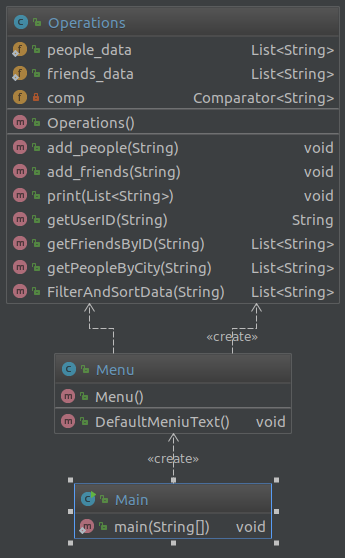
\includegraphics[width=0.5\textwidth]{Class_diagram.png}
\caption{\label{fig:class_dia}Project Class diagram.}
\end{figure}

\subsection{Description of the data structures used in the project}
The main data structures used in the Social Network project are type of Lists: \textbf{people\_data} and \textbf{friends\_data}.
\begin{itemize} 
\item \textbf{people\_data}.
\subitem \textit{Usage}: List is used for storing all the people in the social network.
\subitem \textit{Data type}: String.
\subitem \textit{Access modifiers}: public static
\subitem \textit{Class}: Operations
\subitem \textit{Implementation}: \textbf{public static List\textless{}String\textgreater{} people\_data = new ArrayList\textless{}String\textgreater{}();}
\item \textbf{friends\_data}.
\subitem \textit{Usage}: List is used for storing all the friends clique in the social network.
\subitem \textit{Data type}: String.
\subitem \textit{Access modifiers}: public static
\subitem \textit{Class}: Operations
\subitem \textit{Implementation}: \textbf{public static List\textless{}String\textgreater{} friends\_data = new ArrayList\textless{}String\textgreater{}();}
\end{itemize}
Some Operations class functions have implemented lists data structures in order to store results or display information.

\subsection{Design and implementation of the methods}
\begin{itemize}
\item \textbf{Menu class}:
\subitem  \textbf{public Menu()}: Menu class constructor which invokes Operations class in order to access Social Network functions. Constructor analyze user inputs in order to achieve Social Network functions. The diagram of all available functions which are available for user are displayed in the figure \ref{fig:menu_dia}. Available operations according user input value:
\subsubitem \textbf{input = 0}: Exit the Social Network program.
\subsubitem input = 1: Take the data from a person and add him/her to the network.
This function does not read any data from Console. This function receives the data as
parameters.
\subsubitem \textbf{input = 2}: Upload people's data (people.txt) from a file in our directory
and add them to the social network. Use the function developed in the previous
point.
\subsubitem \textbf{input = 3}: Print out a listing to a text file of the people on the network.
\subsubitem \textbf{input = 4}: The task is to implement an operation that relates
them in the network, that is, the relationship has to be stored in the network.
\subsubitem \textbf{input = 5}: On the social network: given a person surname, retrieve his/her friends.
\subsubitem \textbf{input = 6}: On the social network: given a city, retrieve all people who were born there.
\subsubitem \textbf{input = 7}: On the social network: retrieve the people who were born between dates D1 and D2,
sorted by birthplace, surname, name. The order relationship will be implemented
according to the lexicographic order (dictionary's order) of the strings used for the
attributes.
\begin{figure}[H]
\centering
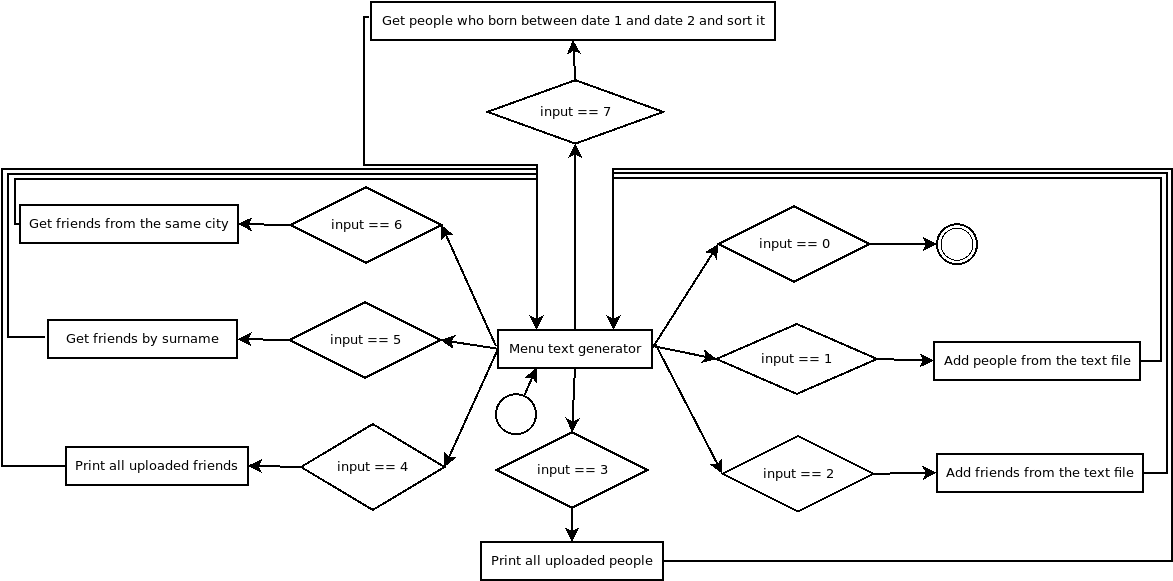
\includegraphics[width=1.2\textwidth]{Menu.png}
\caption{\label{fig:menu_dia} Menu operations scheme.}
\end{figure}
\subitem \textbf{public void DefaultMeniuText()}: This is a void methods which only display text of menu for the user. Menu text in the program can be seen in the figure \ref{fig:menu_text}.
\begin{figure}[H]
\centering
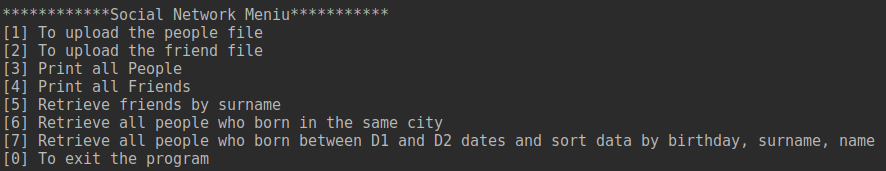
\includegraphics[width=1\textwidth]{menu_text.png}
\caption{\label{fig:menu_text} Displayed default Menu text in the Social Network program.}
\end{figure}
\item \textbf{Operations class}:
\subitem \textbf{public void addPeople(String path)}: This Method is responsible for reading the data of people file using scanner and add the data to the list(friends\_data) data structure. It has one argument: \textbf{String path} which is the path of the people text file in the local computer file system.
\subitem \textbf{public void addFriends(String path)}: This Method responsible for reading the data of friends file using scanner and add the data to the list(friends\_data) data structure. It has one argument: \textbf{String path} which is the path of the friends text file in the local computer file system.
\subitem \textbf{public void print(List<String> data)}: This method prints the data in the terminal of the List. It has one argument: \textbf{List<String> data} - is a list of stored data. In program this method is used for displaying elements of \textbf{people\_data}, \textbf{friends\_data} or other lists which could be created during in operations implementation.
\subitem \textbf{public String getUserID(String surname)}: Method for getting UserID attribute value from people\_data list. This method iterate between every element in people\_data list and search for a surname which is passed from program User. It has one argument: \textbf{String surname} - which is an program user written input text value. 
\subitem \textbf{public List<String> getFriendsByID(String userID)}: Method for displaying all friends of person which UserID attribute matches with given userID. It has one argument: \textbf{String userID} - which is the person code. It returns a list of all person friends surnames.
\subitem \textbf{public List<String> getPeopleByCity(String city)}: Method for displaying all people in the social network which birthday place matches with city text value. It has one argument: \textbf{String city} - which is the city of people birthday place. It returns a list of all person which birthday place text value matches with city text value.
\subitem \textbf{public List<String> getPeopleByCity(String city)}: Method for displaying all people in the social network which birthday place matches with city text value. It has one argument: \textbf{String city} - which is the city of people birthday place. It returns a list of all person which birthday place text value matches with city text value.
\subitem \textbf{public List<String> FilterAndSortData(String date)}: Method for creating new list for storing filtered and sorted people\_data list data. It has one argument: \textbf{String date} - is written date range for filtering in the String data type written as an input from program User. Format of this method date should be like this: \textbf{date = "dd-mm-yyyy dd-mm-yyyy"}; for example: \textbf{date = "12-09-1982 15-04-1992"}. At first date should be less than the second date. Sorting operation is performed after data has been filtered.\\
Filtered data is sorted in ascending way according 3 people data attributes:
\begin{enumerate}
\item \textbf{Person Birthday date}
\item \textbf{Person surname}
\item \textbf{Person name}
\end{enumerate}
\end{itemize}
\bibliographystyle{alpha}
\bibliography{sample}

\end{document}